%%%%%%%%%%%%%%%%%%%%%%%%%%%%%%%%%%
%% HA 1 - 03c Phonologie
%%%%%%%%%%%%%%%%%%%%%%%%%%%%%%%%%%

\begin{frame}%[allowframebreaks]
\frametitle{Hausaufgabe -- Lösung}
\begin{itemize}

\item[1.] Geben Sie eine \textbf{phonetische Transkription} der folgenden Wörter nach der \gqq{Standardaussprache} an, zeichnen Sie dabei die \textbf{Silbestruktur} nach dem \textbf{Konstituentenmodell} und mit der \textbf{Skelettschicht} und geben Sie die \textbf{Sonoritätsprofile} an.

\begin{exe}
\exi{(\ref{ex:03cHA1})}
\begin{xlist}
\ex Stimmenfang
\ex Mittagessen
\ex Bierdeckel
\end{xlist}
\end{exe}

\begin{block}{Sonoritätshierarchie (Zur Erinnerung)}
Vokal $>$ \textipa{/\textscr /} $>$ \textipa{/l/} $>$ Nasal $>$ Frikativ $>$ Plosiv \\
$x > y :=$ $x$ ist sonorer als $y$
\end{block}

\end{itemize}
\end{frame}
%%%%%%%%%%%%%%%%%%%%%%%%%%%%%%%%%%

\begin{frame}{Hausaufgabe -- Lösung}

Zu (\ref{ex:03cHA1a}) Stimmenfang:

\begin{columns}	
	
\column[b]{.5\textwidth}

\begin{figure}
%	\footnotesize
	\centering
	\begin{forest} MyP edges, [, phantom
		[$\sigma$
		[O [x, tier=word [\textipa{S}]] [x, tier=word [\textipa{t}]]]
		[R [N [x, tier=word [\textipa{I}]]] [K [x, name=x [\textipa{m}]]]]
		]
		[$\sigma$
		[O, name=onset]
		[R [N [x [\textipa{@}]]] [K [x [\textipa{n}]]]]
		]
		[$\sigma$
		[O [x, tier=word [\textipa{f}]]]
		[R [N [x [\textipa{a}]]] [K [x [\textipa{N}]]]]
		]
		]				
		{
		\draw[black] (x.north)--(onset.south);
		}
	\end{forest}
\end{figure}

\pause

\column[b]{.5\textwidth}

\begin{figure}
%	\footnotesize
	\centering	
	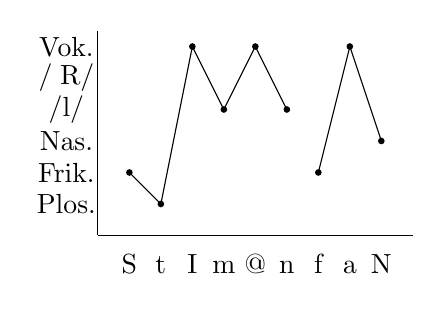
\begin{tikzpicture}[scale=0.4]
		\draw[black] (-1,0) -- (9,0) ; % x axis
		\draw[black] (-1,0) -- (-1,6.5); % y axis
		\node at (-2,1) {Plos.};
		\node at (-2,2) {Frik.};
		\node at (-2,3) {Nas.};
		\node at (-2,4) {\textipa{/l/}};
		\node at (-2,5) {\textipa{/\;R/}};
		\node at (-2,6) {Vok.};
		\draw[black] (0,2) -- (1,1) -- (2,6) -- (3,4) -- (4,6) -- (5,4);
		\draw[black] (6,2) -- (7,6) -- (8,3);
		\node at (0,-1) {\strut \textipa{S}};
		\node at (1,-1) {\strut \textipa{t}};
		\node at (2,-1) {\strut \textipa{I}};
		\node at (3,-1) {\strut \textipa{m}};
		\node at (4,-1) {\strut \textipa{@}};
		\node at (5,-1) {\strut \textipa{n}};
		\node at (6,-1) {\strut \textipa{f}};
		\node at (7,-1) {\strut \textipa{a}};
		\node at (8,-1) {\strut \textipa{N}};
		\fill (0,2) circle [radius=3pt];
		\fill (1,1) circle [radius=3pt];
		\fill (2,6) circle [radius=3pt];
		\fill (3,4) circle [radius=3pt];
		\fill (4,6) circle [radius=3pt];
		\fill (5,4) circle [radius=3pt];
		\fill (6,2) circle [radius=3pt];
		\fill (7,6) circle [radius=3pt];
		\fill (8,3) circle [radius=3pt];
	\end{tikzpicture}
\end{figure}

\end{columns}

\end{frame}


%%%%%%%%%%%%%%%%%%%%%%%%%%%%%%%%%%%%%%%%%%%%%%%
\begin{frame}{Hausaufgabe -- Lösung}


Zu (\ref{ex:03cHA1b}) Mittagessen:

\begin{columns}
	\column[b]{.5\textwidth}
	
\begin{figure}
\footnotesize
\centering
	\begin{forest} MyP edges, [, phantom
		[$\sigma$
		[O [x, tier=word [\textipa{m}]]] 
		[R [N [x, tier=word [\textipa{I}]]] [K [x, name=x1 [\textipa{t}]]]]
		]
		[$\sigma$
		[O, name=onset1]
		[R [N [x [\textipa{a:}, name=a]]
		[x, name=ax]] [K [x [\textipa{k}]]]]
		]
		[$\sigma$
		[O [x, tier=word [\textipa{P}]]]
		[R [N [x [\textipa{E}]]] [K [x, name=x2 [\textipa{s}]]]]
		]
		[$\sigma$
		[O, name=onset2]
		[R [N [x [\textipa{\textsyllabic{n}}]]] [K]
		]
		]]
		{
		\draw[black] (x1.north)--(onset1.south);
		\draw[black] (x2.north)--(onset2.south);
		\draw[black] (a.north)--(ax.south);
		}
	\end{forest}
\end{figure}

\pause
\column[b]{.5\textwidth}

\begin{figure}
	\footnotesize
	\centering
	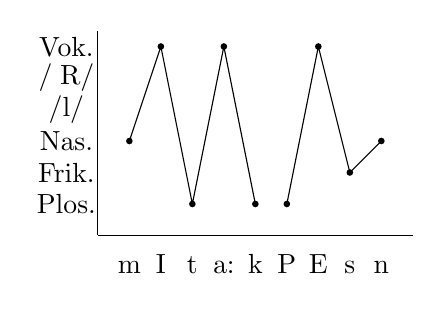
\begin{tikzpicture}[scale=0.4]
		\draw[black] (-1,0) -- (9,0) ; % x axis
		\draw[black] (-1,0) -- (-1,6.5); % y axis
		\node at (-2,1) {Plos.};
		\node at (-2,2) {Frik.};
		\node at (-2,3) {Nas.};
		\node at (-2,4) {\textipa{/l/}};
		\node at (-2,5) {\textipa{/\;R/}};
		\node at (-2,6) {Vok.};
		\draw[black] (0,3) -- (1,6) -- (2,1) -- (3,6) -- (4,1);
		\draw[black] (5,1) -- (6,6) -- (7,2) -- (8,3);
		\node at (0,-1) {\strut \textipa{m}};
		\node at (1,-1) {\strut \textipa{I}};
		\node at (2,-1) {\strut \textipa{t}};
		\node at (3,-1) {\strut \textipa{a:}};
		\node at (4,-1) {\strut \textipa{k}};
		\node at (5,-1) {\strut \textipa{P}};
		\node at (6,-1) {\strut \textipa{E}};
		\node at (7,-1) {\strut \textipa{s}};
		\node at (8,-1) {\strut \textipa{\textsyllabic{n}}};
		\fill (0,3) circle [radius=3pt];
		\fill (1,6) circle [radius=3pt];
		\fill (2,1) circle [radius=3pt];
		\fill (3,6) circle [radius=3pt];
		\fill (4,1) circle [radius=3pt];
		\fill (5,1) circle [radius=3pt];
		\fill (6,6) circle [radius=3pt];
		\fill (7,2) circle [radius=3pt];
		\fill (8,3) circle [radius=3pt];
	\end{tikzpicture}
\end{figure}

\end{columns}

\end{frame}


%%%%%%%%%%%%%%%%%%%%%%%%%%%%%%%%%%%%%%%%%%%%
\begin{frame}{Hausaufgabe -- Lösung}

Zu (\ref{ex:03cHA1b}) Mittagessen (alternative Lösung):

\begin{columns}
	\column[b]{.5\textwidth}
	
	
\begin{figure}
\footnotesize
\centering

	\begin{forest} MyP edges, [, phantom
		[$\sigma$
		[O [x, tier=word [\textipa{m}]]] 
		[R [N [x, tier=word [\textipa{I}]]] [K [x, name=x1 [\textipa{t}]]]]
		]
		[$\sigma$
		[O, name=onset1]
		[R [N [x [\textipa{a:}, name=a]]
		[x, name=ax]] [K [x [\textipa{k}]]]]
		]
		[$\sigma$
		[O [x, tier=word [\textipa{P}]]]
		[R [N [x [\textipa{E}]]] [K [x, name=x2 [\textipa{s}]]]]
		]
		[$\sigma$
		[O, name=onset2]
		[R [N [x [\textipa{@}]]] [K [x [\textipa{n}]]]]
		]
		]
		{
		\draw[black] (x1.north)--(onset1.south);
		\draw[black] (x2.north)--(onset2.south);
		\draw[black] (a.north)--(ax.south);
		}
	\end{forest}

\end{figure}

\pause

\column[b]{.5\textwidth}

\begin{figure}
\footnotesize
\centering
	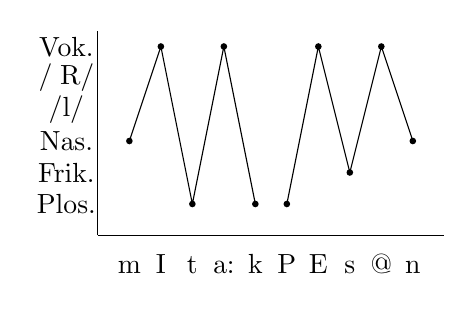
\begin{tikzpicture}[scale=0.4]
		\draw[black] (-1,0) -- (10,0) ; % x axis
		\draw[black] (-1,0) -- (-1,6.5); % y axis
		\node at (-2,1) {Plos.};
		\node at (-2,2) {Frik.};
		\node at (-2,3) {Nas.};
		\node at (-2,4) {\textipa{/l/}};
		\node at (-2,5) {\textipa{/\;R/}};
		\node at (-2,6) {Vok.};
		\draw[black] (0,3) -- (1,6) -- (2,1) -- (3,6) -- (4,1);
		\draw[black] (5,1) -- (6,6) -- (7,2) -- (8,6) -- (9,3);
		\node at (0,-1) {\strut \textipa{m}};
		\node at (1,-1) {\strut \textipa{I}};
		\node at (2,-1) {\strut \textipa{t}};
		\node at (3,-1) {\strut \textipa{a:}};
		\node at (4,-1) {\strut \textipa{k}};
		\node at (5,-1) {\strut \textipa{P}};
		\node at (6,-1) {\strut \textipa{E}};
		\node at (7,-1) {\strut \textipa{s}};
		\node at (8,-1) {\strut \textipa{@}};
		\node at (9,-1) {\strut \textipa{n}};
		\fill (0,3) circle [radius=3pt];
		\fill (1,6) circle [radius=3pt];
		\fill (2,1) circle [radius=3pt];
		\fill (3,6) circle [radius=3pt];
		\fill (4,1) circle [radius=3pt];
		\fill (5,1) circle [radius=3pt];
		\fill (6,6) circle [radius=3pt];
		\fill (7,2) circle [radius=3pt];
		\fill (8,6) circle [radius=3pt];
		\fill (9,3) circle [radius=3pt];
	\end{tikzpicture}
\end{figure}

\end{columns}

\end{frame}


%%%%%%%%%%%%%%%%%%%%%%%%%%%%%%%%%%%%%%%%%%%%%%%
\begin{frame}{Hausaufgabe -- Lösung}

Zu (\ref{ex:03cHA1c}) Bierdeckel:

\begin{columns}
	\column[b]{.5\textwidth}
	
\begin{figure}
\centering
	\begin{forest} MyP edges, [, phantom
		[$\sigma$
		[O [x,tier=word [\textipa{b}]]]
		[R [N [x, tier=word [\textipa{i:}, name=i]] [x,name=x1][x [\textipa{5}]]] [K]
		]
		]
		[$\sigma$
		[O [x, tier=word [\textipa{d}]]]
		[R [N [x [\textipa{E}]]] [K [x, name=x [\textipa{k}]]]]
		]
		[$\sigma$
		[O, name=onset]
		[R [N [x, tier=word [\textipa{@}]]] [K [x [\textipa{l}]]]]
		]
		]
		{
		\draw[black] (x1.south)--(i.north);
		\draw[black] (x.north)--(onset.south);
		}
	\end{forest}
\end{figure}

\pause

\column[b]{.5\textwidth}

\begin{figure}
\centering
	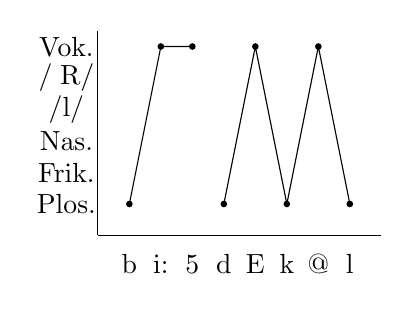
\begin{tikzpicture}[scale=0.4]
		\draw[black] (-1,0) -- (8,0) ; % x axis
		\draw[black] (-1,0) -- (-1,6.5); % y axis
		\node at (-2,1) {Plos.};
		\node at (-2,2) {Frik.};
		\node at (-2,3) {Nas.};
		\node at (-2,4) {\textipa{/l/}};
		\node at (-2,5) {\textipa{/\;R/}};
		\node at (-2,6) {Vok.};
		\draw[black] (0,1) -- (1,6) -- (2,6);
		\draw[black] (3,1) -- (4,6) -- (5,1) -- (6,6) -- (7,1);
		\node at (0,-1) {\strut \textipa{b}};
		\node at (1,-1) {\strut \textipa{i:}};
		\node at (2,-1) {\strut \textipa{5}};
		\node at (3,-1) {\strut \textipa{d}};
		\node at (4,-1) {\strut \textipa{E}};
		\node at (5,-1) {\strut \textipa{k}};
		\node at (6,-1) {\strut \textipa{@}};
		\node at (7,-1) {\strut \textipa{l}};
		\fill (0,1) circle [radius=3pt];
		\fill (1,6) circle [radius=3pt];
		\fill (2,6) circle [radius=3pt];
		\fill (3,1) circle [radius=3pt];
		\fill (4,6) circle [radius=3pt];
		\fill (5,1) circle [radius=3pt];
		\fill (6,6) circle [radius=3pt];
		\fill (7,1) circle [radius=3pt];
	\end{tikzpicture}
\end{figure}

\end{columns}

\end{frame}


%%%%%%%%%%%%%%%%%%%%%%%%%%%%%%%%%%%%%%%%%%%%%%%%%%%
\begin{frame}{Hausaufgabe -- Lösung}

Zu (\ref{ex:03cHA1c}) Bierdeckel (alternative Lösung):

\begin{columns}
	\column[b]{.5\textwidth}
	
	\begin{figure}
		\centering
		\begin{forest} MyP edges, [, phantom
			[$\sigma$
			[O [x,tier=word [\textipa{b}]]]
			[R [N [x, tier=word [\textipa{i:}, name=i]] [x,name=x1][x [\textipa{5}]]] [K]
			]
			]
			[$\sigma$
			[O [x, tier=word [\textipa{d}]]]
			[R [N [x [\textipa{E}]]] [K [x, name=x [\textipa{k}]]]]
			]
			[$\sigma$
			[O, name=onset]
			[R [N [x, tier=word [\textipa{\textsyllabic{l}}]]] [K]
			]
			]
			]
			{
				\draw[black] (x1.south)--(i.north);
				\draw[black] (x.north)--(onset.south);
			}
		\end{forest}
	\end{figure}
	
	\pause
	
	\column[b]{.5\textwidth}
	
	\begin{figure}
		\centering
		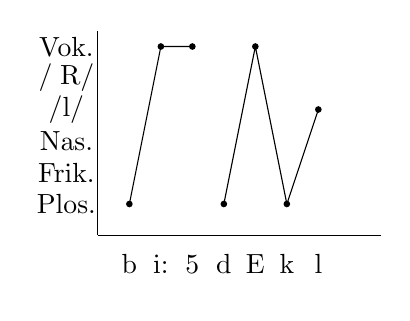
\begin{tikzpicture}[scale=0.4]
		\draw[black] (-1,0) -- (8,0) ; % x axis
		\draw[black] (-1,0) -- (-1,6.5); % y axis
		\node at (-2,1) {Plos.};
		\node at (-2,2) {Frik.};
		\node at (-2,3) {Nas.};
		\node at (-2,4) {\textipa{/l/}};
		\node at (-2,5) {\textipa{/\;R/}};
		\node at (-2,6) {Vok.};
		\draw[black] (0,1) -- (1,6) -- (2,6);
		\draw[black] (3,1) -- (4,6) -- (5,1) -- (6,4);
		\node at (0,-1) {\strut \textipa{b}};
		\node at (1,-1) {\strut \textipa{i:}};
		\node at (2,-1) {\strut \textipa{5}};
		\node at (3,-1) {\strut \textipa{d}};
		\node at (4,-1) {\strut \textipa{E}};
		\node at (5,-1) {\strut \textipa{k}};
		\node at (6,-1) {\strut \textipa{l}};
		\fill (0,1) circle [radius=3pt];
		\fill (1,6) circle [radius=3pt];
		\fill (2,6) circle [radius=3pt];
		\fill (3,1) circle [radius=3pt];
		\fill (4,6) circle [radius=3pt];
		\fill (5,1) circle [radius=3pt];
		\fill (6,4) circle [radius=3pt];
		\end{tikzpicture}
	\end{figure}
	
\end{columns}

\end{frame}


%%%%%%%%%%%%%%%%%%%%%%%%%%%%%%%%%%%%%%%%%%%%%%%%%%
\begin{frame}{Hausaufgabe -- Lösung}
\begin{itemize}
\item[2.] Silbifizieren Sie folgende Segmentsequenzen \textbf{in zwei Schritten}:
\begin{itemize}
\item Onsetmaximierungsprinzip
\item Sonoritätsprinzip
\end{itemize}

Stellen Sie fest, ob alle Silben wohlgeformt sind.\\
Falls nicht, benennen Sie die Verletzungen.

\begin{exe}
\exr{ex:03cHA2} Urinstinkt
\pause
\begin{xlist}
	\settowidth\jamwidth{XXXXXXXXXXXXXXXXXXXXXXXXXXXXXXX}
	\ex \alertred{\textipa{[Pu.\;RI.nStInkt]} \jambox{(Onsetmaximierung)} } \pause
	\ex  \alertred{\textipa{[Pu.\;RIn.(\,S\,)tInkt]} \jambox{(Sonoritätsprinzip, \textipa{S} ist extrasilbisch)} } \pause
	\ex  \alertred{\textipa{[Pu5.PIn.stiNkt]} \jambox{(Silbifizierung der phonologischen Wörter)} }
\end{xlist}
\end{exe}
\pause

\item (\ref{ex:03cHA2}a) und (\ref{ex:03cHA2}b) sind einfach nach der Lautfolge silbifiziert.\\
Silbifizierung erfolgt jedoch auf der Ebene des phonologischen Wortes.\\
Daher werden die phonologischen Wörter \ab{ur-} und \ab{Instinkt} einzeln silbifiziert.
\end{itemize}
\end{frame}

%%%%%%%%%%%%%%%%%%%%%%%%%%%%%%%%%%%%%%%%%%%%%%%%

\begin{frame}{Hausaufgabe -- Lösung}
\begin{itemize}	
\item[3.] Geben Sie die standarddeutsche \textbf{phonetische Transkription} des Wortes \ab{Stahltische} inklusive der \textbf{Silbenstruktur} (mit X-Skelettschicht) an. Ermitteln Sie die \textbf{Kriterien}, die bei der Silbifizierung wirken.
\end{itemize}

\pause

\begin{minipage}{.5\textwidth}
\begin{figure}
\scalebox{.8}{\begin{forest}
MyP edges [, phantom
[$\sigma$
[O 
[x, tier=word[\textipa{S}]]
[x, tier=word[\textipa{t}]]
]
[R
[N
[x, tier=word[\textipa{a:}, name=a]]
[x, name=x]
]
[K[x[\textipa{l}]]]
]
]
[$\sigma$
[O [x, tier=word[\textipa{t}]]]
[R
[N
[x[\textipa{I}]]
]
[K
[x,name=S[\textipa{S}] ]
]
]
]
[$\sigma$
[O, name=o]
[R
[N
[x[\textipa{@}]]
]
]
]
]
\draw[black](o.south)--(S.north);
\draw[black](a.north)--(x.south);
\end{forest}}
\end{figure}
\end{minipage}
\begin{minipage}{.45\textwidth}
	
\pause	
	
\begin{itemize}
\item Onset-Maximierung \pause
\item Sonoritätshierarchie im Onset: *Sonorant vor Obstruent (*[\textipa{lt}]) \pause
\item Silbengelenk nach ungespanntem, betontem Vokal
\end{itemize}
\end{minipage}

\end{frame}

%%%%%%%%%%%%%%%%%%%%%%%%%%%%%%%%%%%%%

\begin{frame}{Hausaufgabe -- Lösung}
\begin{itemize}

\item[4.] Geben Sie die Gründe an, warum die folgenden Wörter aus phonetisch/""phonologischen Gründen im Deutschen nicht möglich sind:

\begin{exe}
	\exr{ex:03cHA3}
	\settowidth\jamwidth{XXXXXXXXXXXXXXXXXXXXXXXXXXXXXXXXXXX}
	\begin{xlist}
		\ex[*]{ \textipa{['Napl.O:t]}
			\loesung{2}{Onset-Maximierung \textipa{[pl]}, \textipa{[N]} steht am Wortanfang,} 
			\loesung{2}{\textipa{[O]} ist ungespannt und lang} }
		\ex[*]{ \textipa{[a\;R.'tUng]}
			\loesung{3}{Auslautverhärtung, regressive velare nasale Assimilation,}\loesung{3}{Knacklaut} }
	\end{xlist}

\end{exe}

\end{itemize}

\end{frame}
